%======================================================================
\subsection{BW-ASM-06 --- Interference \& clearance (planned and built 25 Oct 2026)}\label{sec:asm06-plan}
%======================================================================

You chose this epic on 25 Oct and asked for it to be built on my recommendations. This section records them: what
the command does, the decisions and why, the acceptance test on the Leonardo gearbox, and the questions left for you.
Upstream FreeCAD 1.1 has nothing to reuse: \file{src/Mod/Assembly} has no interference or collision code (one
comment about limits that ``might clash''). What exists here is the section view (\eref{MOD-16}): it paints clashes
red \emph{on its plane}, measures one pair's overlap volume, and keeps \emph{fits}, part pairs whose overlap is
intended. A clash off the plane is not seen. \eref{FND-08} counted 276 pairs on the gearbox, checked by hand.

\paragraph{What it does.} \emph{Inspect $\rightarrow$ Interference} (Design workspace, also in the Assembly menu)
checks the active assembly, or the file's top assembly. It opens a command tab in the right panel
(figure~\ref{fig:asm06-mock}), runs at once, and lists every pair of parts in one of four groups:
\begin{center}
\small
\begin{tabularx}{\linewidth}{@{}l>{\hsize=1.1\hsize}X>{\hsize=0.9\hsize}X@{}}
\toprule
Group & Means & Shown as\\
\midrule
Clash & the parts' material overlaps by more than $\varepsilon_V=10^{-3}$\,mm$^3$ & volume and depth; the overlap drawn
  red over the model\\
Fit & a clash between two parts marked as intended (a screw in its tapped hole, a press fit) & grey; ``Not a fit''
  puts it back\\
Contact & the parts touch (closer than $\varepsilon_d=10^{-4}$\,mm), no volume to speak of & ``touching''; the
  contact point marked\\
Clearance & apart, but closer than the gap you ask for (on, 0.2\,mm: an FDM print's fit) & the distance; a line
  between the nearest points\\
\bottomrule
\end{tabularx}
\end{center}
Picking a row selects both parts and draws the overlap (or the nearest points) on top of the model, so a clash
inside the housing is still seen; \emph{Zoom} frames the pair. \emph{Mark as fit} keeps the pair out of the clashes
from then on, with an optional reason, in this check \emph{and} in every section view of the file.

\begin{figure}[htbp]
\centering
\begin{tikzpicture}[x=1mm,y=1mm,font=\sffamily\scriptsize]
  % the panel
  \draw[rounded corners=2mm, fill=white, draw=black!25] (0,0) rectangle (78,104);
  \node[anchor=west, font=\sffamily\small\bfseries] at (3,99) {Interference};
  \node[anchor=east, text=black!55] at (75,99) {NEMA 17 planetary gearbox 5:1};
  \draw[black!15] (0,95) -- (78,95);
  \node[anchor=west] at (3,91) {\textcolor{bwblue}{$\blacksquare$} Clearance closer than};
  \draw[rounded corners=0.8mm, draw=black!30] (40,88.8) rectangle (56,93.2); \node at (48,91) {0.20 mm};
  \node[anchor=west] at (3,86) {\textcolor{bwblue}{$\blacksquare$} List touching contacts};
  \draw[rounded corners=1mm, fill=bwblue, draw=bwblue] (58,84) rectangle (75,93.5);
  \node[text=white, font=\sffamily\scriptsize\bfseries] at (66.5,88.75) {Check again};
  \node[anchor=west, text=black!55] at (3,80.5) {24 parts, 69 pairs near each other, checked in 5.6 s};
  \draw[black!15] (0,77) -- (78,77);
  % groups
  \node[anchor=west, font=\sffamily\scriptsize\bfseries, text=bwred] at (3,73) {$\blacktriangledown$ Clashes (1)};
  \fill[bwblue!14, rounded corners=0.6mm] (2,66.3) rectangle (76,70.3);
  \node[anchor=west] at (6,68.3) {Sun / Carrier}; \node[anchor=east] at (75,68.3) {257.6 mm$^3$, 2.1 mm deep};
  \node[anchor=west, font=\sffamily\scriptsize\bfseries, text=black!60] at (3,62) {$\blacktriangledown$ Fits (8)};
  \node[anchor=west, text=black!60] at (6,57.5) {Adapter plate / M3x40 1}; \node[anchor=east, text=black!60] at (75,57.5) {8.6 mm$^3$, 0.3 mm deep};
  \node[anchor=west, text=black!60] at (6,53.5) {Motor / M3x6 1}; \node[anchor=east, text=black!60] at (75,53.5) {9.3 mm$^3$, 0.3 mm deep};
  \node[anchor=west, text=black!45] at (6,49.5) {\dots\ 6 more};
  \node[anchor=west, font=\sffamily\scriptsize\bfseries, text=bworange] at (3,45) {$\blacktriangleright$ Clearance (0)};
  \node[anchor=west, font=\sffamily\scriptsize\bfseries, text=black!60] at (3,40) {$\blacktriangleright$ Contacts (29)};
  \draw[black!15] (0,36) -- (78,36);
  % row actions
  \foreach \x/\w/\t in {3/22/Mark as fit, 27/22/Not a fit, 51/24/Zoom to pair} {
    \draw[rounded corners=1mm, draw=black!30] (\x,28) rectangle ({\x+\w},33);
    \node at ({\x+\w/2},30.5) {\t};
  }
  \node[anchor=north west, text width=72mm, text=black!60] at (3,25) {Mark as fit: every pair of these two parts
    (all four M3x40 in the adapter plate) leaves the clashes, here and in the section views. Reason (optional):};
  \draw[rounded corners=0.8mm, draw=black!30] (3,9.5) rectangle (75,14); \node[anchor=west, text=black!45] at (4.5,11.75) {Thread modelled at the tap-drill size};
  \node[anchor=west, text=black!45] at (3,5) {Stop while it runs; Close puts the view back.};
  % the canvas
  \begin{scope}[shift={(84,0)}]
    \draw[rounded corners=2mm, fill=black!3, draw=black!25] (0,0) rectangle (84,104);
    \node at (42,52) {\includegraphics[width=78mm]{fig/interference.png}};
    \node[anchor=north west, text width=78mm, text=black!60] at (3,101) {The pair picked: both parts selected, the
      overlap drawn red over the model (here the bolt of figure~\ref{fig:clash}).};
  \end{scope}
\end{tikzpicture}
\caption{Mock of the Interference tab with the gearbox's numbers (the old sun hub, rev.~1 of \code{LE-01-01009}, put
back to show a real clash; the screws already marked as fits). The canvas shows the bolt example's overlap.}
\label{fig:asm06-mock}
\end{figure}

%----------------------------------------------------------------------
\subsubsection*{Decisions (my recommendations, 25 Oct)}

\begin{center}
\small
\begin{tabularx}{\linewidth}{@{}>{\hsize=0.55\hsize}X>{\hsize=1.45\hsize}X@{}}
\toprule
Decision & Why\\
\midrule
A fit is a pair of \emph{parts}, not of occurrences & The section view already keeps fits that way
  (\code{"Doc\#Part\textbackslash tDoc\#Part"}), so one mark agrees in both places; and a thread fit is a property
  of the two parts: all four M3x40 screws sit in the same tapped holes. The roadmap's earlier note (``filtered by
  occurrence path'') is changed to this.\\
Fits stored on the assembly, copied to every section & The assembly keeps \code{Fits} and \code{FitNotes} (the
  reason). Marking a fit also writes it into each section's \code{Fits}, which the viewer reads; unmarking removes it
  from both. A section made later reads the assembly's fits once \file{bruceworx\_section.py} asks for them (a
  one-line change I leave to the session that owns that file).\\
Hidden parts are left out & As in the section view and in Fusion: what you hide you are not checking. Sub-assemblies
  are opened down to their parts; link arrays count element by element.\\
Contacts listed, collapsed & 29 on the gearbox: useful to confirm that a bearing sits in its bore, noise otherwise. A
  checkbox turns them off.\\
Clearance on, 0.2\,mm & Your parts are printed; 0.2\,mm is a common FDM fit. A gap of exactly the value passes:
  the M3 screws' 0.2\,mm clearance holes in the housing are fine.\\
Depth & How far the overlap reaches into either part:
  $\displaystyle \delta=\max_{p\in\partial(A\cap B)}\max\bigl(d(p,\partial A),\,d(p,\partial B)\bigr)$, sampled on
  the overlap's boundary. The bolt 4\,mm too long gives 4.0; a thread modelled at the tap-drill size gives its radial
  overlap (0.25\,mm for M3 in 2.5\,mm).\\
On the GUI thread, a few pairs at a time & OpenCASCADE's Booleans and distances keep Python's lock, so a thread
  would not keep the window responsive. The check runs in 50\,ms steps with a progress bar and Stop.\\
Nothing existing changes & A new command; the only shared state is the fit marks, changed by you (rule
  \eref{FND-07}).\\
Headless too & \code{bruceworx\_interference.check\_file(path)} returns the counts and pairs as JSON for the release
  check of \eref{PDM-07} (``no clash, or each one waived with a reason'').\\
\bottomrule
\end{tabularx}
\end{center}

%----------------------------------------------------------------------
\subsubsection*{How it is fast enough}

The broad phase sorts the 24 parts' boxes (grown by the gap) along $x$ and sweeps: 276 pairs become 65 to 69
candidates. The narrow phase works per pair on the \emph{faces} that matter. OpenCASCADE's
\code{BRepExtrema\_ShapeProximity} (\code{Shape.proximity} in FreeCAD) finds, on meshes of deflection $\delta$
(0.1\,\% of the part, 0.01--0.2\,mm), the faces of each part that come within $r+2\delta$ of the other, $r$ being
the gap: a true distance $\le r$ is never missed, because each mesh lies within $\delta$ of its surface. Face pairs
are then bounded cheaply (box gap; a plane the other face's box lies to one side of; a bore the other box sits inside
of) and measured exactly with \code{distToShape}, faces on the same plane or cylinder first, since that is where
parts sit on each other. Only pairs whose boundaries touch get the exact Boolean common, which tells a clash from a
contact. A part buried in another has boundaries that never meet; a point-in-solid test finds it. Measured on the
gearbox (headless, 25 Oct, other FreeCADs running): 13.7\,s for the Boolean and the distance of whole parts on the
65 candidates, 8.4\,s measuring only faces near the other part's box, 5.4--5.7\,s with the proximity search. Six gear meshes (sun and ring with each planet) are 3\,s of it: their
Booleans on 150--300-face gears.

%----------------------------------------------------------------------
\subsubsection*{Acceptance test}

\begin{enumerate}[nosep]
  \item The bolt of figure~\ref{fig:clash}: one clash, 78.5\,mm$^3$, 4.0\,mm deep (a unit test).
  \item The gearbox \code{LE-02-01002} (copy): 24 parts, 276 pairs; \textbf{8 clashes}, all thread fits (adapter
    plate / M3x40 $\times4$ at 8.6\,mm$^3$, motor / M3x6 $\times4$ at 9.3\,mm$^3$), \textbf{29 contacts}, no clearance
    below 0.2\,mm (8 below 0.5\,mm); under 10\,s. Marking the two fits leaves 0 clashes and 8 fits, and a section
    through a screw no longer shows it red.
  \item The old sun hub (rev.~1) put back: one more clash, sun / carrier, 257.6\,mm$^3$: the overlap the section
    view found on its plane.
  \item Picking a row selects both parts and draws the overlap; Close leaves the file unchanged except for fits.
\end{enumerate}

%----------------------------------------------------------------------
\subsubsection*{Built (25 Oct)}

\file{bruceworx\_interference.py} (the check, headless) and \file{bruceworx\_interference\_gui.py} (the command and
its tab), with \file{TestBruceWorxInterference.py}: 15 tests headless, 17 in the GUI (the bolt, a thread at the
tap-drill size, contact, clearance and a gap of exactly the value, a part buried in another, hidden parts, links as
occurrences of one part, fits shared with a section, \code{check\_file}, the tab: list, pick, overlay, mark and
unmark, Close). \emph{Interference} is in Design $\rightarrow$ Inspect and in the Assembly menu after \emph{Bill of
Materials}.

\begin{figure}[htbp]
\centering
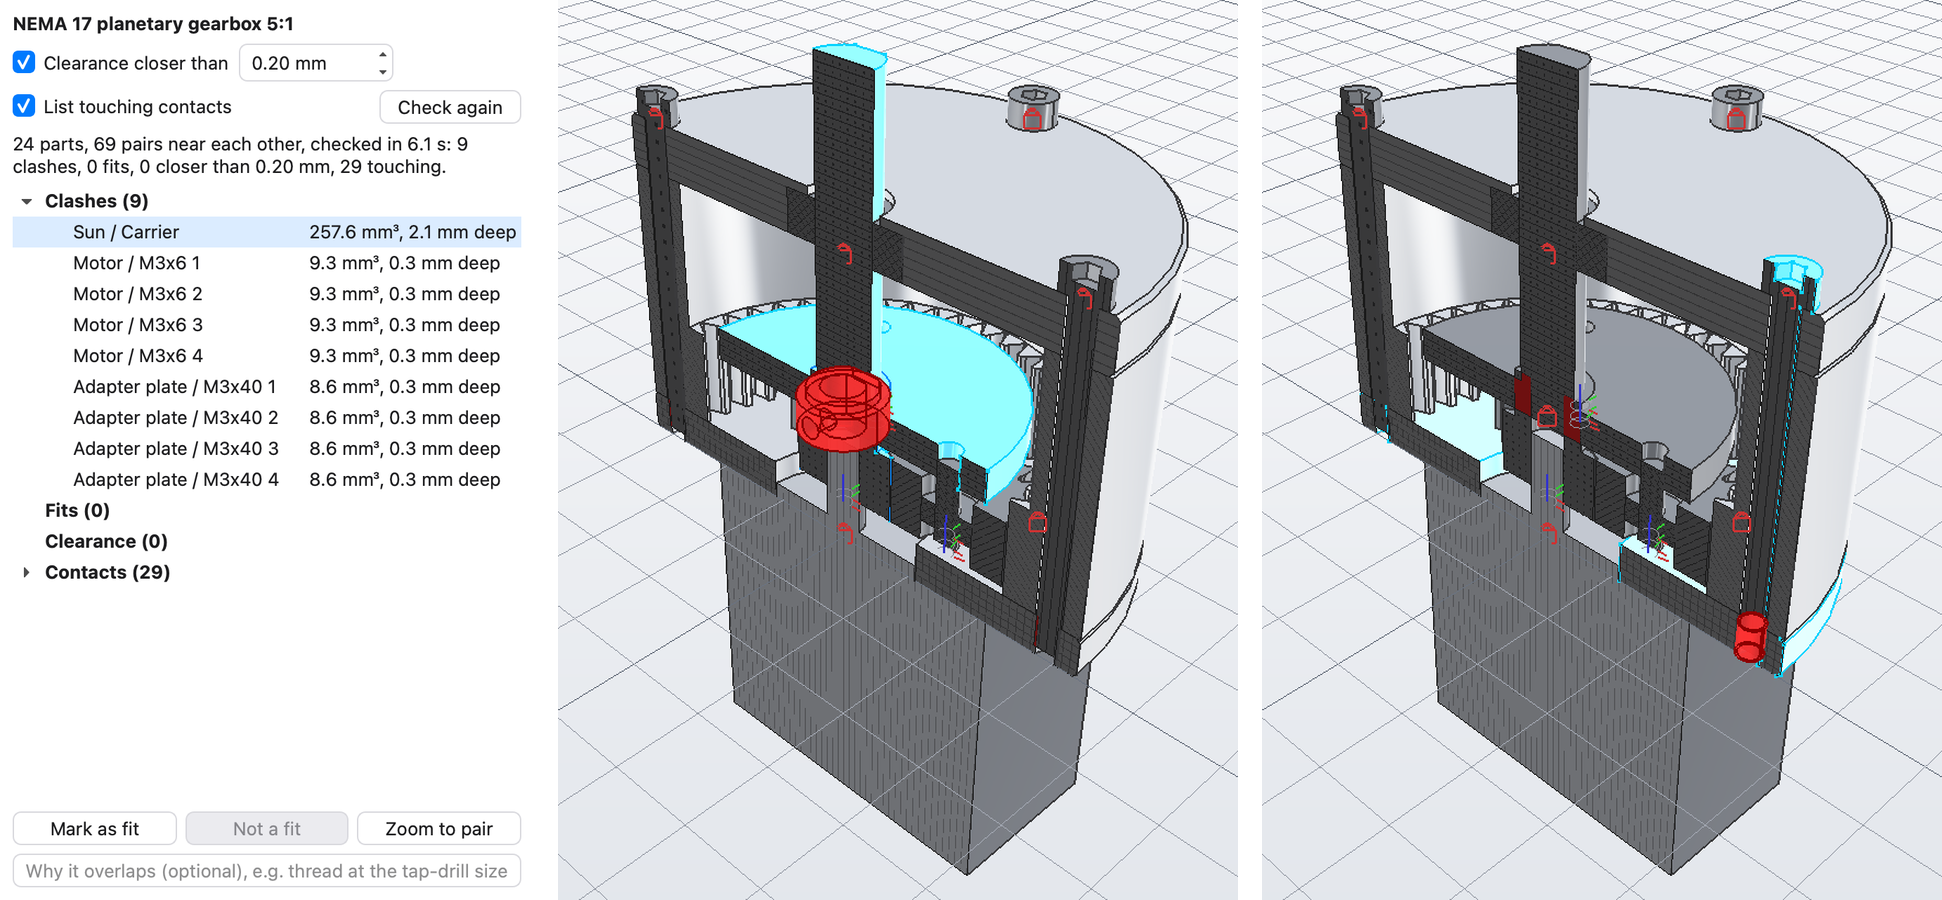
\includegraphics[width=\linewidth]{fig/asm06_built.png}
\caption{Built, on a copy of the gearbox with the old sun hub (rev.~1) put back, with a section through the axis on.
Left: the tab after the check. Middle: \emph{Sun / Carrier} picked: both parts selected, the 257.6\,mm$^3$ overlap
drawn red over the model. Right: after \emph{Mark as fit} on the two thread fits, \emph{Adapter plate / M3x40 1}
picked: its thin overlap at the foot of the screw. The section's own red, at the sun hub, is the clash that is
left.}
\label{fig:asm06-built}
\end{figure}

\begin{center}
\small
\begin{tabularx}{\linewidth}{@{}>{\hsize=0.7\hsize}X>{\hsize=1.3\hsize}X@{}}
\toprule
Acceptance step & Result (25 Oct)\\
\midrule
1. The bolt & One clash, 78.5\,mm$^3$, 4.0\,mm deep (unit test, headless and in the GUI tab).\\
2. The gearbox & 24 parts, 276 pairs, 65 candidates (69 with the 0.2\,mm gap, 75 with 0.5\,mm). 8 clashes, all thread
  fits (adapter plate / M3x40 $\times4$ 8.6\,mm$^3$, motor / M3x6 $\times4$ 9.3\,mm$^3$, each 0.3\,mm deep); 29
  contacts; none closer than 0.2\,mm; 8 closer than 0.5\,mm (the screws in their 0.2\,mm clearance holes). Headless
  5.4--5.7\,s. After \emph{Mark as fit} twice: 0 clashes, 8 fits, both keys on the assembly and in the section's
  \code{Fits}, which the section view passes to the viewer as fits.\\
3. The old sun hub & One more clash, sun / carrier, 257.6\,mm$^3$, 2.1\,mm deep: the volume measured for this clash in
  \S\ref{sec:mod16-plan}. In the GUI: 6.2\,s for the whole check, the view redrawn at least every 0.9\,s (the longest
  step is one gear pair's Boolean).\\
4. Pick and Close & A row selects both occurrences and draws the overlap or the nearest points on top; Close removes
  the drawing and the selection; the undo list holds only the two \emph{Mark as fit} steps.\\
\bottomrule
\end{tabularx}
\end{center}

\paragraph{Left for later.} (1) A section made \emph{after} a fit is marked does not see it until
\file{bruceworx\_section.py}'s \code{style\_of()} also reads \code{bruceworx\_interference.fits(doc)}; a one-line
change for the session that owns that file. (2) The release check of \eref{PDM-07} can call \code{check\_file()};
wiring it in is that epic's. (3) A cache, so a check after moving one part only measures the pairs it is in. (4)
\eref{ECD-04}'s board-in-housing fit is this check on the enclosure assembly.

%----------------------------------------------------------------------
\subsubsection*{Questions for you}

\begin{enumerate}[nosep]
  \item Fits per part pair (all four screws at once), as recommended, or per occurrence?
  \item Should the release check fail on clearance below the gap too, or only on clashes that are not fits?
  \item Leave hidden parts out (recommended), or check everything in the assembly?
  \item Is 0.2\,mm the right default gap, and should it live on the assembly (saved with the file) rather than in
    your preferences?
\end{enumerate}
